\section{Evaluation Metrics}
\label{sec:clustering_agent_representation_metrics}

To evaluate the effectiveness of \gls{car}, four evaluation metrics are introduced:

\begin{itemize}
    \item \textbf{\BehaviorReconstructionName} : it measures how well a surrogate policy faithfully reproduces the behavior of the initial policy by comparing their cumulative rewards.
    \item \textbf{\ClusteringUniversalityName} : it evaluates the stability of clusterings by measuring the similarity of clusters obtained from independently trained surrogate policies.
    \item \textbf{\AbstractionScoreName} : it quantifies the extent to which \gls{ls} clusters capture abstractions rather than directly reflecting the structure of observations, actions, or the network architecture prior to training.
    \item \textbf{\AdjustedClusteringUniversalityName} : it combines the two previous metrics into a single measure of how much of the cross-seed agreement captured by \ClusteringUniversalityName cannot be explained away by any of the trivial baselines underlying \AbstractionScoreName.
\end{itemize}

The remainder of this section details the motivation for each metric and describes how they are calculated.
In the first subsection, we develop the \BehaviorReconstructionName{}.
We then introduce the \gls{ari} measure, which serves as the foundation for the three other metrics introduced in the subsequent subsections, namely \ClusteringUniversalityName{}, \AbstractionScoreName{}, and \AdjustedClusteringUniversalityName{}.

\subsection{Behavior Reconstruction}

% We argue that explaining a function $b$ that closely approximates another function $a$ is essentially the same as explaining $a$.
% If $b$ accurately captures the key decision patterns of $a$, understanding $b$ provides meaningful insights into how $a$ works \cite{guidotti2018surveymethodsexplainingblack}.
% In our setting, this means that generating explanations for $\SurrogatePolicy{}$ that faithfully reproduce $\InitialPolicy$ amounts to explaining $\InitialPolicy$ directly.

We introduce the \BehaviorReconstructionName metric to assess whether $\SurrogatePolicy{}$ faithfully reproduces the behavior of $\InitialPolicy$.
This metric compares the returns obtained by the initial policy $\InitialPolicy$ and the surrogate policies $\SurrogatePolicy{}$ over a set of evaluation episodes.
We use the definition of return introduced in Section~\ref{subsec:value_functions}, where $g(t,\gamma)$ denotes the discounted sum of rewards collected along a trajectory $t$.
Here, the return is computed over complete episodes with $\gamma=1$, so $g$ corresponds to the total reward collected during the episode.
Each policy is evaluated over $m$ episodes.
We denote by $g_{\InitialPolicy}^{i}$ the return obtained by the initial policy in episode $i$, and by $g_{\SurrogatePolicy{j}}^{i}$ the return obtained by surrogate policy $\SurrogatePolicy{j}$ in episode $i$.
The \BehaviorReconstructionName{} is then defined as the mean return of the surrogate policies normalized by the mean return of the initial policy:

\begin{align}
    \text{\BehaviorReconstructionName} = \frac{1}{n \sum_{i=1}^{m} g_{\InitialPolicy}^{i}} \sum_{j=1}^{n} \sum_{k=1}^{m} g_{\SurrogatePolicy{j}}^{k}
\end{align}

In imitation learning, it is unlikely to expect the surrogate policy $\SurrogatePolicy{}$ to outperform the initial policy $\InitialPolicy$ it aims to approximate through supervised learning \cite{pmlr-v9-ross10a}.
Consequently this metric ranges in $[0,1]$.
Values approaching 1 indicate minimal loss in reproducing $\InitialPolicy$, while values close to 0 indicate poor reproduction.  

We deliberately adopt a reward-based definition rather than alternatives based on actions or action distributions (e.g., training loss, accuracy, KL divergence \cite{shlens2014noteskullbackleiblerdivergencelikelihood}, or optimal transport \cite{peyré2020computationaloptimaltransport}).
Since surrogate policies are trained in a supervised manner, they cannot develop strategies beyond those demonstrated by the initial policy.
This means that if the rewards achieved are comparable, the surrogate policy is effectively copying the initial policy's behavior.

\subsection{Adjusted Rand Index}
\label{subsec:adjusted_rand_index}

Within \gls{car}, concepts are assumed to correspond to clusters in the \gls{ls}.
Combined with the \RepresentationConvergenceHypothesisName, this leads to a direct experimental prediction.
If independently trained surrogate policies converge toward the same conceptual organization, clustering their \gls{lr} should produce similar partitions.

When a particular observation is processed by the network, it is expected to activate the same concept regardless of the specific neural implementation of the policy.
If independently trained policies converge toward the same conceptual organization, a given observation should activate the same concept across all models.
As a consequence, observations grouped together within a cluster for one policy should also be grouped together for another independently trained policy.

In the clustering literature, the most used measures for comparing two partitions is the \gls{ari}~\cite{hubert1985comparing}.
This measure quantifies the agreement between cluster assignments independently of the spatial organization of the clusters.
Both metrics introduced later in this chapter, \ClusteringUniversalityName{} and \AbstractionScoreName{}, rely on the \gls{ari}.
Since the \gls{ari} is a complex measure, we review its definition and discuss its main properties.

The \gls{ari} is derived from the \gls{ri}~\cite{rand1971objective}, which measures the agreement between two partitions by considering every possible pair of points in the point cloud.
For each pair, four situations are possible:
\begin{itemize}
\item \textbf{Agreement:} The points belong to the same cluster in both partitions.
\item \textbf{Agreement:} The points belong to different clusters in both partitions.
\item \textbf{Disagreement:} The points belong to the same cluster in the first partition but to different clusters in the second.
\item \textbf{Disagreement:} The points belong to different clusters in the first partition but to the same cluster in the second.
\end{itemize}

The \gls{ri} measures the proportion of pairs for which the two partitions agree:
$$
\text{RI} = \frac{\text{number of agreeing pairs}}{\text{total number of pairs}}.
$$

Although the \gls{ri} is intuitive, it suffers from an important limitation.
In most clustering problems, the majority of pairs of points belong to different clusters.
Consequently, even two completely independent partitions will agree on a large number of pairs, simply because both assign them to different clusters.
This effect becomes more pronounced as the number of points or clusters increases.

The \gls{ari} addresses this issue by accounting for the agreement that would be expected purely by chance.
It compares the observed agreement $\text{RI}$ to the expected agreement under random partitions $\mathbb{E}[\text{RI}]$.
The score is then normalized by the maximum agreement achievable beyond this random baseline, $\max(\text{RI}) - \mathbb{E}[\text{RI}]$.
As a result, an \gls{ari} of $0$ corresponds to the level of agreement expected from random clusterings, while an \gls{ari} of $1$ indicates perfect agreement between the two partitions:
\[
\text{ARI} = \frac{\text{RI} - \mathbb{E}[\text{RI}]}{\max(\text{RI}) - \mathbb{E}[\text{RI}]}
\]

In practice, the \gls{ari} is computed directly from the cluster assignments of the two partitions.
Let clustering \(A\) be composed of partitions \(\{A_i\}\) and clustering \(B\) of partitions \(\{B_j\}\).
Let \(a_i = |A_i|\) denote the number of samples in partition \(i\) of clustering \(A\), and \(b_j = |B_j|\) the number of samples in partition \(j\) of clustering \(B\).
Furthermore, let \(n_{ij} = |A_i \cap B_j|\) be the number of samples shared by partition \(i\) of clustering \(A\) and partition \(j\) of clustering \(B\), and let \(n\) be the total number of samples.
With these definitions, the \gls{ari} can be computed as:

\[
\text{ARI} =
\frac{
\sum_{i,j} \binom{n_{ij}}{2}
-
\left[
\sum_i \binom{a_i}{2}
\sum_j \binom{b_j}{2}
\right]
\big/ \binom{n}{2}
}{
\frac{1}{2}
\left[
\sum_i \binom{a_i}{2}
+
\sum_j \binom{b_j}{2}
\right]
-
\left[
\sum_i \binom{a_i}{2}
\sum_j \binom{b_j}{2}
\right]
\big/ \binom{n}{2}
}
\]

Because it is bounded by $1$, a value such as $0.5$ can be misleadingly interpreted as ``halfway to a perfect match.''
This interpretation is incorrect because the \gls{ari} is normalized against the agreement expected from two random partitions.
As a result, values close to $1$ require the two clusterings to be nearly identical, while a value of $0.5$ already indicates substantial agreement~\cite{amezquita2020orchestrating}.

\subsection{Clustering Universality}
\label{subsec:clustering_universality}

Having introduced the \gls{ari}, we can now define the \ClusteringUniversalityName metric.
While the \gls{ari} quantifies the similarity between two partitions, the objective of \gls{car} is to assess the consistency of conceptual organizations across an entire set of independently trained surrogate policies.

To this end, the same set of observations is projected into the \gls{ls} of each surrogate policy and clustered.
Under the \RepresentationConvergenceHypothesisName, these independently obtained partitions are expected to be similar.
\ClusteringUniversalityName{} quantifies this by computing the mean pairwise \gls{ari}:

\begin{align}
    \text{\ClusteringUniversalityName}
    =
    \frac{1}{\binom{n}{2}}
    \sum_{i=2}^{n}
    \sum_{j=1}^{i-1}
    \operatorname{ARI}(\mathcal{C}_{i}, \mathcal{C}_{j}).
\end{align}

This metric takes values in $[-1, 1]$.
A value close to $1$ indicates that surrogate policies produce highly similar partitions, suggesting that the clusters reflect intrinsic properties of the policy.
Conversely, a value near $0$ implies that the similarity between partitions is no better than that of two randomly generated clusterings, meaning that the clustering fails to capture any meaningful structure in the policy.
A negative value, on the other hand, signals that the agreement between partitions is worse than what would be expected by chance, indicating a systematic disagreement between the clusterings.

Figure~\ref{fig:clustering_universality_illustration} illustrates \ClusteringUniversalityName{} in the ideal case.
It shows three \gls{ls} obtained by projecting the same seven observations, labeled 1 to 7, through three independently trained surrogate policies.
Although the embeddings occupy different positions, the clusters group exactly the same elements in all three cases.
The partitioning is therefore identical, resulting in an \gls{ari} of $1$.

% --- Macro pour une surrogate policy + son ensemble ---
\newcommand{\surrogatepolicy}[7]{%
    % #1 : xshift
    % #2 : index (1,2,3,…)
    % #3 : liste des coordonnées X des points
    % #4 : liste des coordonnées Y des points
    % #5 : liste des coordonnées X des circlepattern
    % #6 : liste des coordonnées Y des circlepattern
    % #7 : liste des diamètres des circlepattern
    \node[policybox] (policy#2) at (#1,0)
        {\scalebox{2}{$\textcolor{myred}{\pi}^{\textcolor{myred}{'}}_{\textcolor{myred}{#2}}$}};

    \begin{scope}[xshift=#1, yshift=-4cm, scale=0.8, transform shape]
        \node[pointset] (box#2) at (0,0) {};
        \begin{scope}
            \clip (box#2.south west) rectangle (box#2.north east);
            % Circlepattern avec diamètres spécifiques
            \foreach \cx/\cy [count=\i] in {#5} {
                \pgfmathsetmacro{\currentcy}{{#6}[\i-1]}
                \pgfmathsetmacro{\diameter}{{#7}[\i-1]}
                \node[draw, dashed, circle, minimum size=\diameter] at (\cx cm, \currentcy cm) {};
            }
        \end{scope}

        % Points avec E_i dans un cercle bleu
        \foreach \x/\y [count=\i] in {#3} {
            \pgfmathsetmacro{\currenty}{{#4}[\i-1]}
            \node[draw=myblue, circle, inner sep=2pt, fill=white] at (\x cm, \currenty cm) {\scalebox{0.8}{\textcolor{myblue}{\small $\i$}}};
        }
    \end{scope}
    \draw[->, dashed, preaction={draw=white,line width=6pt}] (policy#2) -- ($(box#2.north)+(0,0)$);
}

\begin{figure}[t]
    \centering
    \resizebox{\textwidth}{!}{
    \begin{tikzpicture}[
        policybox/.style={
            draw, rectangle, text centered,
            minimum height=1cm, minimum width=2.5cm,
            align=center, rounded corners=0.2cm
        },
        pointset/.style={
            draw, minimum width=4cm, minimum height=4cm
        },
        circlepattern/.style={
            draw, dashed, circle, minimum width=1.5cm, minimum height=1.5cm
        }
    ]

    % --- Utilisation de la macro pour les trois policies ---
    \surrogatepolicy
    {-6cm}
    {1}
    {-1.5, -1.25, -1, 1.35, 1.0, -0.25, 0.25}
    {-0.75, -1.5, -1, 0.5, 0.0, 1.6, 1.6}
    {-1.25, 1.2, 0}
    {-1.1, 0.2, 1.75}
    {1.5cm, 1.25cm, 1.25cm}

    \surrogatepolicy
    {0cm}
    {2}
    {1, 1.3, 1.5, 0.1, 0.25, 0.45, 1.2}
    {1.5, 1, 1.5, 0.75, 0.2, -1.5, -1}
    {1.25, 0.1, 0.8}
    {1.3, 0.4, -1.2}
    {1.3cm, 1.2cm, 1.6cm}

    \surrogatepolicy
    {6cm}
    {3}
    {0.0, -0.5, 0.25, -1, -1.5, 1.6, 1.2}
    {0.0, 0.5, 0.5, -1.5, -1, 1.2, 1.6}
    {-1.25, -0.15, 1.5}
    {-1.25, 0.3, 1.5}
    {1.3cm, 1.5cm, 1.3cm}

    % --- Acolade et équation en dessous ---
    \draw[
        line width=1pt,  % Épaisseur du trait
        decorate,
        decoration={
            brace,
            amplitude=20pt,  % Hauteur de l'acolade
            mirror,          % Acolade sous la ligne
            raise=10pt       % Décalage vertical
        }
    ]
        (-8.5, -5.5) -- (8.5, -5.5);

    \node[below=0.75cm] at (0, -6) {
        \scalebox{1.5}{$\displaystyle
        \text{\ClusteringUniversalityName} = \frac{1}{\binom{n}{2}} \sum_{i=1}^{n} \sum_{j=0}^{i-1} \operatorname{ARI}(\mathcal{C}_{i}, \mathcal{C}_{j})
        $}
    };

    \end{tikzpicture}
    }
    \caption{Three point clouds obtained by projecting the same observations through three independently trained surrogate policies $\textcolor{myred}{\pi'_1}$, $\textcolor{myred}{\pi'_2}$, and $\textcolor{myred}{\pi'_3}$. The numbered circles 1 to 7 denote the same seven observations across the three point clouds, and the dashed contours denote the clusters recovered in each latent space.}
    \label{fig:clustering_universality_illustration}
\end{figure}


\subsection{Abstraction Score}
\label{subsec:abstraction_score}

If \ClusteringUniversalityName is high, it becomes important to determine what underlies this stability.
Two possibilities arise:
\begin{enumerate}[label=(\roman*), ref=(\roman*)]
    \item \label{i} the \gls{ls} offers no abstraction, as defined in Definition~\ref{def:abstraction}, either because it merely reproduces the structure of the observation space or action distribution, or because it reproduces a structure that is already present in the network architecture prior to any training;
    \item \label{ii} the \gls{ls} captures similarities in decision-making processes, yielding behaviorally meaningful clusters.
\end{enumerate}

To distinguish among these cases, we introduce the \AbstractionScoreName.
This metric contextualizes latent clusterings by examining how their patterns align with three reference baselines: the raw observation data, the action data, and an untrained network of the same architecture.
We consider : $\mathcal{C}_{obs}$, the clustering in the observation space $\mathbb{O}$, and $\mathcal{C}_{act}$, the clustering in the action-space distribution parameters.
The clusterings $\mathcal{C}_{obs}$ and $\mathcal{C}_{act}$ are performed using the same algorithm, distance metric, and hyperparameters as those used for $\mathcal{C}_{i}$ in the \gls{ls}, ensuring that any biases introduced by the clustering procedure itself are minimized.

The third baseline addresses the case where the \gls{ls} merely reflects an inductive bias of the network architecture rather than something learned.
To this end, we introduce $m$ untrained networks sharing the same architecture as the surrogate policies, but with randomly initialized, never-updated weights.
Each of these $m$ untrained networks is used to project the same observations into its own latent space, which is then clustered in the same way, yielding partitions $\mathcal{C}_{untr, 1}, \dots, \mathcal{C}_{untr, m}$.
This baseline isolates what the architecture already imposes on the representation before any learning takes place, so that a high similarity between $\mathcal{C}_i$ and this baseline indicates that the corresponding structure cannot be attributed to training.

For each latent clustering $\mathcal{C}_{i}$, we define its similarity to these three baselines using the \gls{ari}:

\begin{align*}
A^{obs}_{i} &= \operatorname{ARI}(\mathcal{C}_{i}, \mathcal{C}_{obs}) \\
A^{act}_{i} &= \operatorname{ARI}(\mathcal{C}_{i}, \mathcal{C}_{act}) \\
A^{untr}_{i} &= \frac{1}{m} \sum_{k=1}^{m} \operatorname{ARI}(\mathcal{C}_{i}, \mathcal{C}_{untr, k})
\end{align*}

The \AbstractionScoreName is subsequently calculated as one minus the average of the maximum absolute similarity values across these three reference baselines:

\begin{align}
\scalebox{0.9}{%
$\text{\AbstractionScoreName} = 1 - \frac{1}{n} \sum_{i=1}^{n} \max \left( \left|A^{obs}_{i}\right|, \left|A^{act}_{i}\right|, \left|A^{untr}_{i}\right| \right)$%
}
\end{align}

The \AbstractionScoreName ranges from $[0, 1]$.
A score around $0$ means that the latent clusters are strongly aligned with the observation space, the action space, or the untrained network, reflecting no abstraction, case~\ref{i}.
A score close to $1$ indicates that the latent clusters are independent of the observation space, the action space, and the network's initialization, capturing abstractions that meaningfully reflect the agent's behavior, case~\ref{ii}.

\subsection{Adjusted Clustering Universality}
\label{subsec:adjusted_clustering_universality}

As discussed above, \ClusteringUniversalityName alone does not indicate whether the recovered structure is meaningful.
We therefore introduce the \AdjustedClusteringUniversalityName, which measures how much of the agreement between the different surrogate policies remains after accounting for the three trivial baselines.

\begin{align}
\scalebox{0.7}{%
$\text{\AdjustedClusteringUniversalityName} = \text{\ClusteringUniversalityName} - \frac{1}{n} \sum_{i=1}^{n} \max \left( \left|A^{obs}_{i}\right|, \left|A^{act}_{i}\right|, \left|A^{untr}_{i}\right| \right)$%
}
\end{align}

This metric ranges in $[-1, 1]$.
A value close to $1$ indicates that surrogate policies converge toward a partition that is both highly reproducible across seeds and clearly not explained by the observation space, the action space, or the network's initialization, providing the strongest evidence for \RepresentationConvergenceHypothesisName.
A value close to $0$, or negative, indicates that whatever agreement exists between independently trained surrogate policies is largely trivial: the surrogate policies converge, but toward a partition that could just as easily emerge from raw pixel similarity, from the action taken, or from an untrained network sharing the same architecture.

% The results of applying \gls{car} and these metrics to concrete environments are presented in Chapter~\ref{chap:experiments}.